\documentclass[main.tex]{subfiles}
\begin{document}

\chapter{Results}

\section{State transfer optimisation}
Graph of final fidelities

The optimisation converges for pulse lengths \SI{10}{\nano\second}? and above while dropping 

\begin{figure}
    \centering
    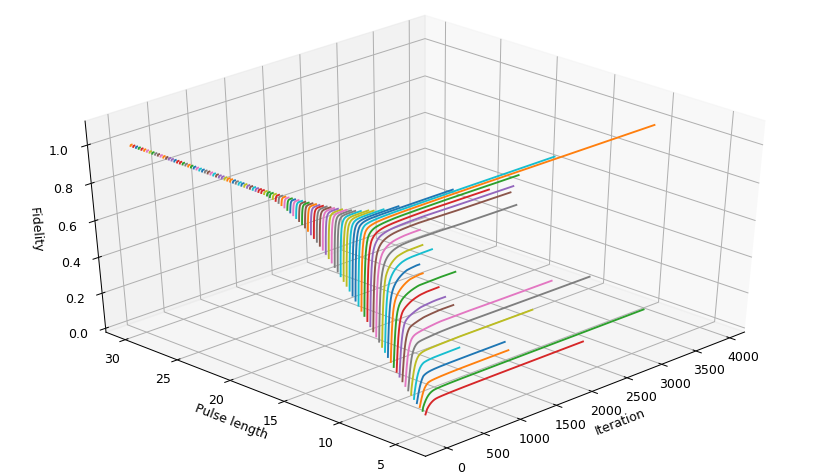
\includegraphics[width=\linewidth]{figs/3d-optim-ge.png}
    \caption{Caption}
    \label{fig:3d-optim-ge}
\end{figure}

\begin{figure}
    \centering
    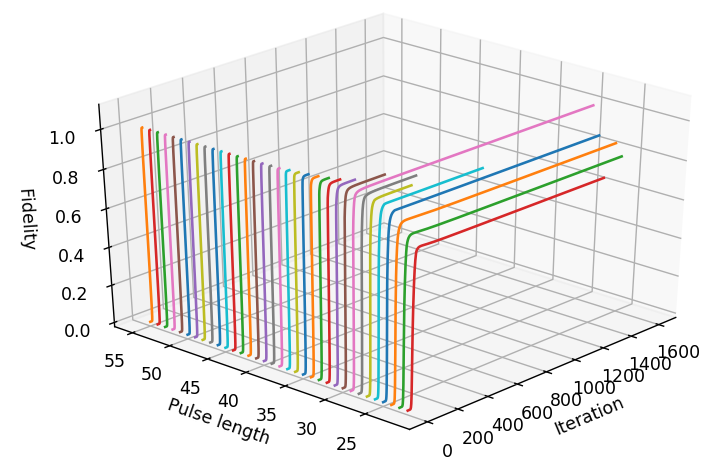
\includegraphics[width=0.7\linewidth]{figs/3d-optim-gf.png}
    \caption{Caption}
    \label{fig:3d-optim-gf}
\end{figure}

\tikzfig{figs/fidelity-length-ge}{Text}{fig:fidelity-length}{15em}{15em}
\tikzfig{figs/fidelity-length-gf}{Text}{fig:fidelity-length2}{15em}{15em}

\tikzfig{figs/pulse_spectrum_30,0}{Text}{fig:fidelity-length}{15em}{15em}

\begin{figure}
    \centering
    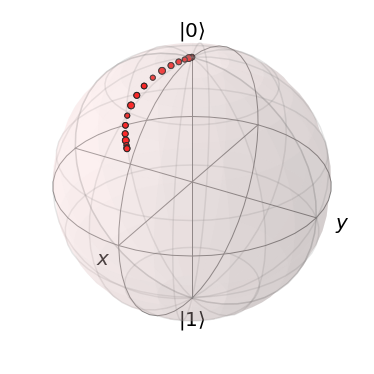
\includegraphics[width=15em]{figs/bloch_evolution_4,25.png}
    \caption{Caption}
    \label{fig:my_label}
\end{figure}

\end{document}
